\documentclass[abstracton,12pt]{scrartcl}
    
\usepackage[utf8]{inputenc}
% \usepackage[T1]{fontenc}
\usepackage{fancyhdr}
\usepackage{graphicx}
\usepackage{tikz}
\usepackage{listings}
\usepackage{amssymb}
\usepackage{amsfonts}
\usepackage{amsmath}
\usepackage{amsthm}
\usepackage{pdfpages}
\usepackage{forest}
\usepackage{multicol}
\usepackage{varwidth}
\usepackage{verbatim}
%\usepackage{minted}
\usepackage{framed}
\usepackage[ruled,vlined]{algorithm2e}
\usepackage{caption}
\usepackage{subcaption}
\usepackage{cleveref}
\usepackage{soul}
% \usepackage{geometry}
% \usepackage{titlesec}

% \forestset{qtree/.style={for tree={parent anchor=south, child anchor=north,align=left,inner sep=0pt}}}
\graphicspath{
  {images/},
  {images/1_unprod_nodes/},
  {images/2_unprod_nodes_tau/}
  {images/3_unprod_nodes_L/}
}

% \setlength{\multicolsep}{6.0pt plus 2.0pt minus 1.5pt}% 50% of original values
% \titleformat{\chapter}{}{\thechapter}{}{}
% \titlespacing{\chapter}{-100pt}{-100pt}{-100pt}

% --------- 

\titlehead{Department of Informatics, University of Zürich}
\subject{\vspace*{2cm}BSc Thesis}
\title{An Adaptive Index for Hierarchical Distributed Database Systems}
\author{
    Rafael Kallis\\[-5pt]
    \scriptsize Matrikelnummer: 14-708-887\\[-5pt]
    \scriptsize Email: \texttt{rk@rafaelkallis.com}
}
\date{\vspace*{2cm}February 1, 2018}
\publishers{
    \small supervised by Prof.\ Dr.\ Michael\ Böhlen and Kevin\ Wellenzohn \\[5cm]
    \begin{tikzpicture}[overlay]
    \node at (-3,-3) {
\includegraphics[height=1.5cm]{IFIlogo}};
    \node at (7,-3) {
\includegraphics[height=1.5cm]{dbtgBW}};
    \end{tikzpicture}
}

% \dedication{dedicated to xxx}

% --------- 

\theoremstyle{definition}

\newtheorem{definition}{Definition}
% \newtheorem{figure}{Figure}
\newtheorem{example}{Example}
% \newtheorem{theorem}{Theorem}
% \newtheorem{lemma}{Lemma}

\crefname{algocfline}{algorithm}{algorithms}
\Crefname{algocfline}{Algorithm}{Algorithms}

\crefname{figure}{Fig.}{Figs.}
\Crefname{figure}{Figure}{Figures}

\crefname{example}{Ex.}{Ex.}
\Crefname{example}{Example}{Examples}

% \newenvironment{proof}
%     {\noindent{\bf Proof:\rm}}{\hfill$\Box$\vspace{\medskipamount}}

\newenvironment{centerverbatim}{\par\centering\varwidth{\linewidth}\verbatim}
    {\endverbatim\endvarwidth\par}

% \def\bbbr{{\rm I\!R}}
% \def\bbbm{{\rm I\!M}}
% \def\bbbn{{\rm I\!N}}
% \def\bbbz{{\rm I\!Z}}

\definecolor{shadecolor}{rgb}{0.97,0.97,0.97}
    
\begin{document}

\maketitle

% \chapter*{Acknowledgements}

% \chapter*{Zusammenfassung}

\newpage

% \tableofcontents
\listoffigures
% \listoftables

\newpage

% \begin{abstract}
%   Frequently adding and removing data from hierarchical indexes causes them to
%   repeatedly grow and shrink. A single insertion or deletion can trigger a
%   sequence of structural index modifications (node insertions/deletions) in a
%   hierarchical index. Skewed and update-heavy workloads trigger repeated
%   structural index updates over a small subset of nodes to the index.

%   Informally, a frequently added or removed node is called \textit{volatile}.
%   Volatile nodes deteriorate index update performance due to two reasons.
%   First, frequent structural index modifications are expensive since they
%   cause many disk accesses. Second, frequent structural index modifications
%   also increase the likelihood of conflicting index updates by concurrent
%   transactions. Conflicting index updates further deteriorate update
%   performance since concurrency control protocols need to resolve the
%   conflict.


% \end{abstract}

\section{Introduction}

Frequently adding and removing data from hierarchical indexes causes them to
repeatedly grow and shrink. A single insertion or deletion can trigger a
sequence of structural index modifications (node insertions/deletions) in a
hierarchical index. Skewed and update-heavy workloads trigger repeated
structural index updates over a small subset of nodes to the index.

Informally, a frequently added or removed node is called \textit{volatile}.
Volatile nodes deteriorate index update performance due to two reasons. First,
frequent structural index modifications are expensive since they cause many disk
accesses. Second, frequent structural index modifications also increase the
likelihood of conflicting index updates by concurrent transactions. Conflicting
index updates further deteriorate update performance since concurrency control
protocols need to resolve the conflict.

Wellenzohn et al.~\cite{KW17} propose the Workload-Aware Property Index (WAPI).
The WAPI exploits the workloads' skewness by identifying and not removing
volatile nodes from the index, thus significantly reducing the number of
expensive structural index modifications. Since fewer nodes are
inserted/deleted, the likelihood of conflicting index updates by concurrent
transactions is reduced.

When the workload characteristics change, new index nodes can become volatile
while others cease to be volatile and become \textit{unproductive}. Unproductive
index nodes slow down queries as traversing an unproductive node is useless,
because neither the node itself nor any of its descendants contain an indexed
property and thus cannot yield a query match. Additionally, unproductive nodes
occupy storage space that could otherwise be reclaimed. lf the workload changes
frequently, unproductive nodes quickly accumulate in the index and the query
performance deteriorates over time. Therefore, unproductive nodes must be
cleaned up to keep query performance stable over time and reclaim disk space as
the workload changes.

Wellenzohn et al.~\cite{KW17} propose periodic Garbage Collection (GC), which
traverses the entire index subtree and prunes all unproductive index nodes at
once. Additionally we propose Query-Time Pruning (QTP), an incremental approach
to cleaning up unproductive nodes in the index. The idea is to turn queries into
updates. Since Oak already traverses unproductive nodes as part of query
processing, these nodes could be pruned at the same time. In comparison to GC,
with QTP only one query has to traverse an unproductive node, while subsequent
queries can skip this overhead and thus perform better.

The goal of this BSc thesis is to study, implement, and empirically compare GC
and QTP as proposed by \cite{KW17} in Apache Jackrabbit Oak (Oak).

% The goal of this project is to implement a WAPI, as proposed by \cite{KW17} in
% Apache Jackrabbit Oak (Oak) in order to improve the transactional throughput
% of Oak. In \Cref{sec:wapi} we describe how nodes are inserted, queried and
% deleted from the WAPI. Next, we describe how volatility is computed in
% \Cref{sec:volatility}. Finally, a reference implementation in Java is
% presented in \Cref{sec:implementation}.

\section{Background}

\subsection{Apache Jackrabbit Oak (Oak)}

% Oak\footnote{https://jackrabbit.apache.org/oak/} is a hierarchical distributed
% database system which makes use of a hierarchical index.
Oak is a hierarchical distributed database system which makes use of a
hierarchical index. Multiple transactions can work concurrently by making use of
Multiversion Concurrency Control (MVCC)~\cite{GW02}, a commonly used optimistic
concurrency control technique~\cite{TM11}.

\Cref{fig:architecture} depicts Oak's multi-tier architecture. Oak embodies the
\textit{Database Tier}.
% Whilst Oak is responsible for handling the database logic, it stores the
% actual data on MongoDB labeled as \textit{Persistence Tier}.
Whilst Oak is responsible for handling the database logic, it stores the actual
data on MongoDB\footnote{https://www.mongodb.com/what-is-mongodb}, labeled as
\textit{Persistence Tier}. On the other end, applications can make use of Oak as
shown in \Cref{fig:architecture} under \textit{Application Tier}.
% One such application is Adobe's enterprise content management system (CMS),
% the Adobe Experience Manager
One such application is Adobe's enterprise content management system (CMS),
the Adobe Experience
Manager\footnote{http://www.adobe.com/marketing-cloud/experience-manager.html}.

\begin{figure}[h]
  \begin{center}
    \begin{tikzpicture}[scale=0.7,thick]
	    \node (mongo) at (0, 0) {
\includegraphics[width = 0.7cm]{MONGO}}; \node
      (oak_a) at (-2, 2) {
\includegraphics[width = 0.7cm]{OAK}}; \node (oak_b)
      at (0, 2) {
\includegraphics[width = 0.7cm]{OAK}}; \node (oak_c) at (2, 2)
      {
\includegraphics[width = 0.7cm]{OAK}}; \node (app_a) at (-2, 4)
      {
\includegraphics[width = 0.7cm]{AEM}}; \node (app_b) at (0, 4)
      {
\includegraphics[width = 0.7cm]{AEM}}; \node (app_c) at (2, 4)
      {
\includegraphics[width = 0.7cm]{AEM}}; \node (mongo_desc) at (5, 0)
      {\footnotesize \textit{Persistence Tier}}; \node (oak_desc) at (5, 2)
      {\footnotesize \textit{Database Tier}}; \node (mongo_desc) at (5, 4)
      {\footnotesize \textit{Application Tier}}; \foreach \from/\to in
      {app_a/oak_a, app_b/oak_b, app_c/oak_c, oak_a/mongo, oak_b/mongo,
        oak_c/mongo} \draw [->] (\from) -- (\to);
    \end{tikzpicture}
  \end{center}
  % \vspace{-0.5cm}
  \caption{Apache Jackrabbit Oak's system architecture}
  \label{fig:architecture}
\end{figure}

\subsection{Workload Aware Property Index (WAPI)}
\label{sec:wapi}

The WAPI is hierarchically organized under node \texttt{/i} (denoted
\textit{Index Subtree Root} in \Cref{fig:hierarchical_db}).
The second index level consists of all properties $k$ we want
to index. The third index level contains any values $v$ of property $k$.
The remaining index levels replicate all nodes from the root node to any
content node with $k$ set to $v$. We denote node $n$'s property $k$ as
$n[k]$ and node $n$'s desendants as $desc(n)$. Given index node $n$, we denote
$n$'s corresponding content node as $*n$.

\begin{definition}
  (Matching Node) Node $n$, with path \texttt{/i/k/v/m}, is matching
  iff $n$'s corresponding content node $*n$, with path \texttt{/m}, has property
  $k$ set to $v$, i.e
  $$ matching(n) \iff *n[k] = v $$
  \label{def:matching_node}
\end{definition}

We also assign property $m = \top$ to a matching index node for the reader's convenience.

% \begin{definition}
%   (Matching Set): Node $n$ is a member the matching set 
%   iff $n$, or any descendant of $n$, is matching, i.e
%   $$ n \in \widehat{matching}\iff \exists m( m \in \{n\} \cup desc(n) \land matching(m)) $$
% \end{definition}

Oak mostly executes content-and-structure (CAS) queries~\cite{CM15}, defined as
follows.

\begin{definition}
  (CAS-Query): Given node $m$, property $k$ and value $v$, a CAS query
  $Q(k,v,m)$ returns all descendants of $m$ which have $k$ set to $v$, i.e
  $$ Q(k,v,m) = \{ n | n \in desc(m) \land matching(n)\} $$
\end{definition}

\begin{figure}
  \centering
  \scriptsize{
    \begin{forest}
      [
      [$\lambda:i$
      [$\lambda:x$
      [$\lambda:1$
      [$\lambda:a$
      [$\lambda:b$
      [$\lambda:d$ \\ $m:\top$, align=center, base=bottom, name=i_node] {
        \draw[<-,gray] (.north west)--++(-5em,1em)
        node[anchor=east]{\textit{Matching Node}};
      }
      ]
      [,phantom]
      ]
      ]
      ]
      ] {
        \draw[<-,gray] (.south west)--++(-5em, -1em)
        node[anchor=east]{\textit{Index Subtree Root}};
      }
      [$\lambda:a$
      [$\lambda:b$
      [$\lambda:d$ \\ $x:1$, align=center, base=bottom, name=c_node]
      ]
      [$\lambda:c$
      [$\lambda:e$]
      ]
      ] {
        \draw[<-,gray] (.south east)--++(5em, -1em)
        node[anchor=west]{\textit{Content Subtree Root}};
      }
      ]
      \draw[->,dotted] (i_node) to[out=east, in=south] node[gray,midway,right]{\textit{corresponding content node}} (c_node);
    \end{forest}
  }
  \caption{An instance of an hierarchical database}
  \label{fig:hierarchical_db}
\end{figure}

\begin{example}
  Consider \Cref{fig:hierarchical_db}. The subtree rooted at \texttt{/a} is
  the content subtree. The subtree rooted at \texttt{/i} is the index
  substree. Node \texttt{/i/x/1/a/b/d} is matching, since its corresponding
  content node, \texttt{/a/b/d}, has property $x$ set to $1$. CAS-Query
  $Q(x,1,\texttt{/a})$, which queries for every descendant of \texttt{/a} with
  $x$ set to $1$, would evaluate to $Q(x,1,\texttt{/a}) = \{\texttt{/a/b/d}\}$,
  since \texttt{/a/b/d} is the only descendant of \texttt{/a} with $x$ set to $1$. 
\end{example}

The WAPI is an hierarchical index and indexes the properties of nodes in order
to answer CAS-queries efficiently. Additionally, it takes into account if an
index node is volatile before performing structural index modifications. If a
node is considered volatile, we do not remove it from the index.

Volatility is the measure which is used by the WAPI in order to distinguish
when to remove a node or not from the index.
Wellenzohn et al.~\cite{KW17} propose to look at the recent transactional
workload to check whether a node $n$ is volatile. The workload on Oak instance
$O_i$ is represented by a sequence $H_i = \langle \ldots, G^a, G^b, G^c
\rangle$ of snapshots, called a history. Let $t_n$ be the current time and
$t(G^b)$ be the point in time snapshot $G^b$ was committed, $N(G^a)$ is the
set of nodes which are members of snapshot $G^a$. We use a superscript $a$
to emphasize that a node $n^a$ belongs to tree $G^a$. $pre(G^b)$ is the
predecessor of snapshot $G^b$ in $H_i$.

Node $n$ is volatile iff $n$'s volatility count is at least $\tau$, called
volatility threshold. The volatility count of $n$ is defined as the number of
times $n$ was added or removed from snapshots in a sliding window of length
$L$ over history $H_i$.

Given two snapshots $G^a$ and $G^b$ we write $n^a$ and $n^b$ to emphasize that
nodes $n^a$ and $n^b$ are two versions of the same node $n$, i.e, they have
the same absolute path from the root node.

\begin{definition}
  (Volatility Count): The volatility count $vol(n)$ of node $n$ is the number of
  times node $n$ was added or removed from snapshots contained in a sliding
  window of length $L$ over history $H_i$.
  \begin{align*}
    % \begin{split}
    vol(n) = | \{ G^b | G^b \in H_i \land t(G^b) \in [t_{n-L+1}, t_n] \land \exists G^a[ \\
    \qquad G^a = pre(G^b) \land ([n^a \notin N(G^a) \land n^b \in N(G^b)]\lor \\
    \qquad [n^a \in N(G^a) \land n^b \notin N(G^b)] )]\} |
    % \end{split}
  \end{align*}
  \label{def:vol_count}
\end{definition}

\begin{definition}
  (Volatile Node): Node $n$ is volatile iff $n$'s volatility count (see
  \Cref{def:vol_count}) is greater or equal than the volatility threshold
  $\tau$, i.e
  $$ volatile(n) \iff vol(n) \geq \tau $$
  \label{def:volatile_node}
\end{definition}

% \begin{definition}
%   (Volatile Set): Node $n$ is a member the volatile set
%   iff $n$, or any descendant of $n$, is volatile, i.e
%   $$ n \in \widehat{volatile}\iff \exists m( m \in \{n\} \cup desc(n) \land volatile(m)) $$
% \end{definition}

% Note that the matching and volatile sets are not mutually exclusive.

\section{Unproductive Nodes}

When time passes and the database workload changes, volatile nodes cease to be
volatile and they become unproductive.

\begin{definition}
  (Unproductive Node): Node $n$ is unproductive iff $n$, and any descendant of
  $n$, is neither matching (see \Cref{def:matching_node}) nor volatile (see
  \Cref{def:volatile_node}), i.e
  $$ unproductive(n) \iff \nexists m (m \in (\{n\} \cup desc(n)) \land
  (matching(m) \lor volatile(m)))$$
\end{definition}

\begin{example}
  Consider the snapshots depicted in \Cref{fig:unproductive_nodes}. Assume volatility
  threshold $\tau = 1$, sliding window length $L = 1$ and history $H_h
  = \langle G^0,G^1,G^2,G^3,G^4,G^5,G^6 \rangle$. Oak instance $O_h$ executes transactions
  $T_1, \dots , T_6$. Snapshot $G^0$ was committed at time $t(G^0) =
  t$. Given snapshot $G^0$, transaction $T_1$ adds property $x=1$ to
  \texttt{/a/b/d} and commits snapshot $G^1$ at time $t(G^1) = t + 1$. Next,
  transaction $T_2$ removes property $x$ from \texttt{/a/b/d} given snapshot
  $G^1$ and commits snapshot $G^2$ at time $t(G^2) = t + 2$. The index nodes are
  not pruned during $T^2$ since they are volatile. Transaction $T_3$ adds
  property $x=1$ to \texttt{/a/c/e} given $G^2$ and commits $G^3$ at time
  $t(G^3) = t+3$. % Notice how 
  \texttt{/i/x/1/a/b/d} and \texttt{/i/x/1/a/b} are
  the only unproductive index nodes and \texttt{/i/x/1/a/c/e} is the only
  volatile index node in $G^3$. % Transaction
  % $T^4$ again adds property $x=1$ to \texttt{/a/b/d} given snapshot $G^3$ and
  % commits snapshot $G^4$ at time $t(G^4) = t+4$. In $G^4$, nodes
  % \texttt{/i/x/1/a/b/d} and \texttt{/i/x/1/a/b} are not unproductive anymore
  % since \texttt{/i/x/1/a/b/d}'s content node is matching. Transaction $T^5$
  % again removes property $x$ from \texttt{/a/b/d} given snapshot $G^4$ and
  % commits snapshot $G^5$ at time $t(G^5) = t+5$. Since nodes
  % \texttt{/i/x/1/a/b/d} and \texttt{/i/x/1/a/b} are not volatile, they are
  % pruned from the property index during $T^5$. Finally transaction $T^6$ removes
  % property $x=1$ from \texttt{/a/c/e} given snapshot $G^5$ and commits snapshot
  % $G^6$ at time $t(G^6) = t+6$. Index nodes \texttt{/i/x/1/a/c/e} and
  % \texttt{/i/x/1/a/c} are pruned from the property index during $T^6$ because
  % they are not volatile.
\end{example}

\begin{figure}[h]
  \centering
  \begin{large}
  $$ G^0 \xrightarrow{\quad T_1 \quad} G^1 \xrightarrow{\quad T_2 \quad} G^2
  \xrightarrow{\quad T_3 \quad} G^3%  \xrightarrow{\quad T_4 \quad} G^4
  % \xrightarrow{\quad T_5 \quad} G^5 \xrightarrow{\quad T_6 \quad} G^6
  $$
\end{large}

\begin{subfigure}{0.24\textwidth}
  \centering \scriptsize{
    \begin{framed}
      \begin{forest}
        [
        [$\lambda:i$
        [,phantom]
        ]
        [$\lambda:a$
        [$\lambda:b$
        [$\lambda:d$]
        ] 
        [$\lambda:c$
        [$\lambda:e$]
        ]
        ]
        ]
      \end{forest}

      \vspace{28mm}
    \end{framed}
  } \footnotesize{ Snapshot $G^0$
 
    $t(G^0) = t$ }
\end{subfigure}
\begin{subfigure}{0.24\textwidth}
  \centering \scriptsize{
    \begin{framed}
      \begin{forest}
        [
        [$\lambda:i$
        [$\lambda:x$
        [$\lambda:1$
        [$\lambda:a$
        [$\lambda:b$
        [$\lambda:d$ \\ $m:\top$, align=center, base=bottom]
        ]
        [,phantom]
        ]
        ]
        ]
        ]
        [$\lambda:a$
        [$\lambda:b$
        [$\lambda:d$ \\ $x:1$, align=center, base=bottom]
        ]
        [$\lambda:c$
        [$\lambda:e$]
        ]
        ]
        ]
      \end{forest}
    \end{framed}
  } \footnotesize{ Snapshot $G^1$
 
    $t(G^1) = t+1$ }
\end{subfigure}
\begin{subfigure}{0.24\textwidth}
  \centering \scriptsize{
    \begin{framed}
      \begin{forest}
        [
        [$\lambda:i$
        [$\lambda:x$
        [$\lambda:1$
        [$\lambda:a$
        [$\lambda:b$
        [$\lambda:d$]
        ]
        [,phantom]
        ]
        ]
        ]
        ]
        [$\lambda:a$
        [$\lambda:b$
        [$\lambda:d$]
        ]
        [$\lambda:c$
        [$\lambda:e$]
        ]
        ]
        ]
      \end{forest}

      \vspace{4.2mm}
    \end{framed}
  } \footnotesize{ Snapshot $G^2$
 
    $t(G^2) = t+2$ }
\end{subfigure}
\begin{subfigure}{0.24\textwidth}
  \centering \scriptsize{
    \begin{framed}
      \begin{forest}
        [
        [$\lambda:i$
        [$\lambda:x$
        [$\lambda:1$
        [$\lambda:a$
        [$\lambda:b$
        [$\lambda:d$]
        ]
        [$\lambda:c$
        [$\lambda:e$ \\ $m:\top$, align=center, base=bottom]
        ]
        ]
        ]
        ]
        ]
        [$\lambda:a$
        [$\lambda:b$
        [$\lambda:d$]
        ]
        [$\lambda:c$
        [$\lambda:e$ \\ $x:1$, align=center, base=bottom]
        ]
        ]
        ]
      \end{forest}
    \end{framed}
  } \footnotesize{ Snapshot $G^3$
 
    $t(G^3) = t+3$ }
\end{subfigure}

% \vspace{5mm}

% \begin{subfigure}{0.24\textwidth}
%   \centering \scriptsize{
%     \begin{framed}
%       \begin{forest}
%         [
%         [$\lambda:i$
%         [$\lambda:x$
%         [$\lambda:1$
%         [$\lambda:a$
%         [$\lambda:b$
%         [$\lambda:d$ \\ $x:1$, align=center, base=bottom]
%         ]
%         [$\lambda:c$
%         [$\lambda:e$ \\ $x:1$, align=center, base=bottom]
%         ]
%         ]
%         ]
%         ]
%         ]
%         [$\lambda:a$
%         [$\lambda:b$
%         [$\lambda:d$ \\ $x:1$, align=center, base=bottom]
%         ]
%         [$\lambda:c$
%         [$\lambda:e$ \\ $x:1$, align=center, base=bottom]
%         ]
%         ]
%         ]
%       \end{forest}
%     \end{framed}
%   } \footnotesize{ Snapshot $G^4$
 
%     $t(G^4) = t+4$ }
% \end{subfigure}
% \begin{subfigure}{0.24\textwidth}
%   \centering \scriptsize{
%     \begin{framed}
%       \begin{forest}
%         [
%         [$\lambda:i$
%         [$\lambda:x$
%         [$\lambda:1$
%         [$\lambda:a$
%         [$\lambda:c$
%         [$\lambda:e$ \\ $x:1$, align=center, base=bottom]
%         ]
%         ]
%         ]
%         ]
%         ]
%         [$\lambda:a$
%         [$\lambda:b$
%         [$\lambda:d$]
%         ]
%         [$\lambda:c$
%         [$\lambda:e$ \\ $x:1$, align=center, base=bottom]
%         ]
%         ]
%         ]
%       \end{forest}
%     \end{framed}
%   } \footnotesize{ Snapshot $G^5$
 
%     $t(G^5) = t+5$ }
% \end{subfigure}
% \begin{subfigure}{0.24\textwidth}
%   \centering \scriptsize{
%     \begin{framed}
%       \begin{forest}
%         [
%         [$\lambda:i$
%         [,phantom]
%         ]
%         [$\lambda:a$
%         [$\lambda:b$
%         [$\lambda:d$]
%         ]
%         [$\lambda:c$
%         [$\lambda:e$]
%         ]
%         ]
%         ]
%       \end{forest}

%       \vspace{28mm}
%     \end{framed}
%   } \footnotesize{ Snapshot $G^6$
 
%     $t(G^6) = t+6$ }
% \end{subfigure}

\vspace{3mm}
\caption*{
  Given $\tau = 1$, $L = 1$, nodes \texttt{/i/x/1/a/b/d} and \texttt{/i/x/1/a/b}
  are unproductive in snapshot $G^3$. They are not volatile and don't match either.
}
\caption{Unproductive Nodes Example}
\label{fig:unproductive_nodes}
\end{figure}

\subsection{Impact on Query Execution Runtime}

In this section we will study and quantify the impact of unproductive nodes on
query runtime. Informally, we call \textit{Query Execution Runtime} the time
needed for a query to finish processing. We hypothesize that unproductive nodes
significantly slow down queries under specific workloads. During query
execution, traversing an unproductive node is
useless, because neither the node itself nor any of its descendants contains
an indexed property and therefore cannot contribute a query match.
An index under a \textit{job-queue} like,
changing workload (see \textbf{forward reference}) is dominated by unproductive nodes.

We formalize the statements above into the following hypotheses:

\begin{shaded}
  \begin{itemize}
  \item[$H_1$:] Average query execution runtime increases under a job-queue
    like, changing workload with the WAPI.
  \item[$H_2$:] Unproductive nodes significantly affect average query execution
    runtime under a job-queue like, changing worload with the WAPI.
  \end{itemize}
\end{shaded}

In order to find supporting evindence for the hypotheses above, a series of
experiments was conducted on Oak. The experimental evaluation and the used
datasets will be described in a later section (\textbf{forward reference}). We
recorded  the query execution runtime throughout the experiment and present the data below.

\Cref{fig:query_runtime_synthetic_millis,fig:query_runtime_aem_millis} show the
recorded query runtime over time as observed from the synthetic and AEM dataset respectively. 
\Cref{fig:query_runtime_synthetic_updates,fig:query_runtime_aem_updates} show the
recorded query runtime over update operations from the synthetic and AEM dataset respectively. 
We observe an increase of the runtime from $2 ms$ to $38 ms$
after running the simulation for $5$ minutes ($2 \cdot 10^4$ update operations)
on the synthetic dataset.

\begin{figure}[h]
  \centering
  \begin{subfigure}{0.49\linewidth}
    \centering
    Synthetic
  \end{subfigure}
  \begin{subfigure}{0.49\linewidth}
    \centering
    AEM
  \end{subfigure}
    \begin{subfigure}{0.49\linewidth}
    \centering
    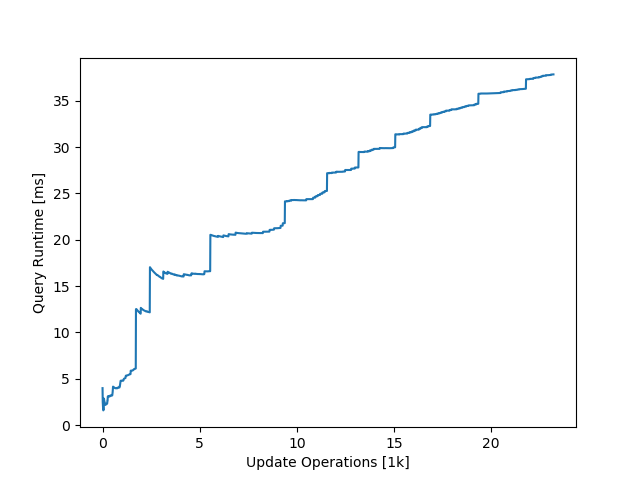
\includegraphics[width=8cm]{updates_query_runtime}
    \caption{}
    \label{fig:query_runtime_synthetic_updates}
  \end{subfigure}
  \begin{subfigure}{0.49\linewidth}
    \centering
    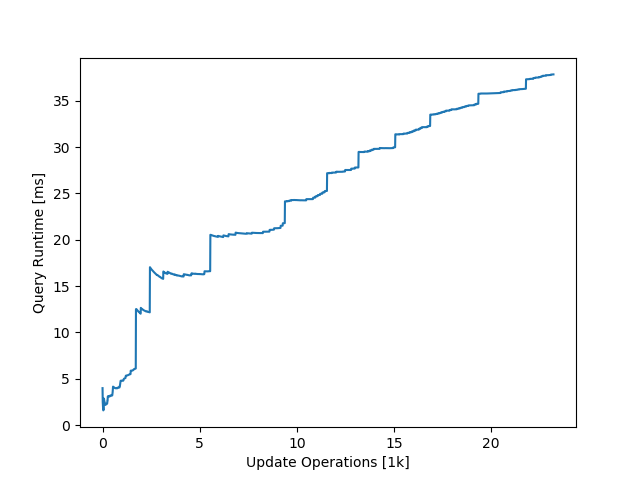
\includegraphics[width=8cm]{updates_query_runtime}
    \caption{}
    \label{fig:query_runtime_aem_updates}
  \end{subfigure}
  \caption{Query Execution Runtime}
  \label{fig:query_runtime}
\end{figure}

Next, we present data regarding the type of nodes encountered during index traversal while
executing a query.
\Crefrange{fig:trav_nodes_synthetic_millis}{fig:trav_nodes_aem_updates} depict
the number of traversed volatile and unproductive index nodes encountered during query
execution with respect to time and update operations from our datasets.
Since the sliding window length $L$ is set to $30$ seconds, we encounter no
unproductive nodes during the first $30$ seconds of the simulation. Once we
reach the $30$ second mark, our queries encounter unproductive nodes. We observe
two findings. First, we see a descend in volatile nodes. Second, we see a
significant increase in unproductive nodes. Towards the end of the simulation,
we observe the traversed nodes being dominated by unproductive nodes. 

\begin{figure}[h]
  \centering
  \begin{subfigure}{0.49\linewidth}
    \centering
    Synthetic
  \end{subfigure}
  \begin{subfigure}{0.49\linewidth}
    \centering
    AEM
  \end{subfigure}
  \begin{subfigure}{0.49\linewidth}
    \centering
    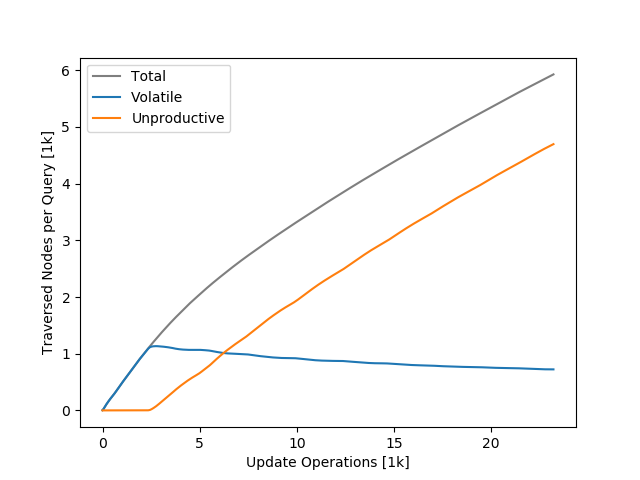
\includegraphics[width=8cm]{updates_traversed_index_nodes}
    \caption{}
    \label{fig:trav_nodes_synthetic_updates}
  \end{subfigure}
  \begin{subfigure}{0.49\linewidth}
    \centering
    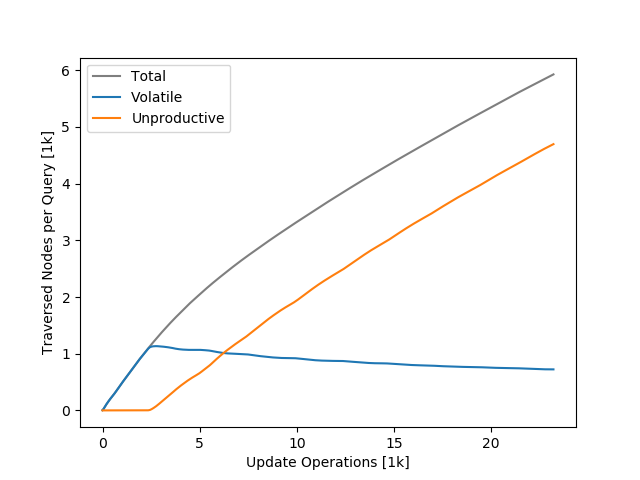
\includegraphics[width=8cm]{updates_traversed_index_nodes}
    \caption{}
    \label{fig:trav_nodes_aem_updates}
  \end{subfigure}
  \caption{Index Structure during Query Execution}
\end{figure}

\begin{figure}[h]
 \centering
  \begin{subfigure}{0.49\linewidth}
    \centering
    Synthetic
  \end{subfigure}
  \begin{subfigure}{0.49\linewidth}
    \centering
    AEM
  \end{subfigure}
  \begin{subfigure}{0.49\linewidth}
    \centering
    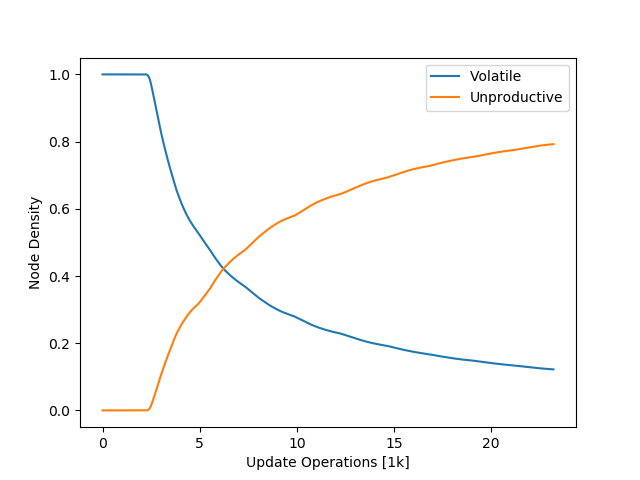
\includegraphics[width=8cm]{updates_index_node_density}
    \caption{}
    \label{fig:trav_node_density_synthetic_updates}
  \end{subfigure}
  \begin{subfigure}{0.49\linewidth}
    \centering
    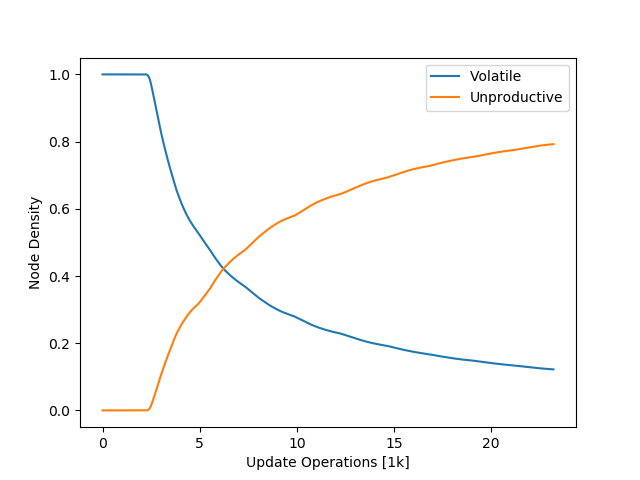
\includegraphics[width=8cm]{updates_index_node_density}
    \caption{}
    \label{fig:trav_node_density_aem_updates}
  \end{subfigure}
 \caption{Node Ratio during Query Execution}
\end{figure}

\Crefrange{fig:trav_node_density_synthetic_millis}{fig:trav_node_density_aem_updates}
show the density of volatile and unproductive nodes over time and update
operations from our datasets. These figures quantify how strongly unproductive
nodes dominate the traversed nodes. The data shows that unproductive nodes
account for over $80\%$ of the traversed nodes whilst less than $20\%$ are volatile. 
Interestingly, we see the density functions to converge towards a value above
$0.8$ and below $0.2$ respectively.

In the following sections we will study the effect of \textit{Volatility
  Threshold $\tau$} and \textit{Sliding Window Length $L$} on query execution runtime and
unproductive nodes.

\subsection{Volatility Threshold $\tau$}

Volatility threshold $\tau$ determines after how many insertions/deletions of an index node
it becomes volatile \cite{KW17}. In this section, we study the impact of
volatility threshold $\tau$ on unproductive nodes and query execution runtime.

We hypothesize that an increase in $\tau$ yields a decrease to the number of traversed unproductive
nodes during query execution. If $\tau$ increases, it is less likely for a node to become
volatile. Having less volatile nodes should imply a decrease in unproductive nodes.

An increase in $\tau$ yields a decrease to the query execution runtime. Less
unproductive nodes should decrease the number of nodes traversed
during query execution and therefore decrease query execution runtime.

An increase in $\tau$ yields a decrease to the unproductive node density during
query execution.

\textbf{Why?}

\begin{shaded}
  \begin{itemize}
  \item[$H_3$:] An increase in $\tau$ yields a decrease to the number of
    traversed unproductive nodes during query execution.
  \item[$H_4$:] An increase in $\tau$ yields a decrease to the query execution runtime. 
  \item[$H_5$:] An increase in $\tau$ yields a decrease to the unproductive node
    density during query execution runtime.
  \end{itemize}
\end{shaded}

The same experiment was conducted under a varying volatility threshold. The
results seem to verify our hypotheses.
\Cref{fig:query_runtime_taus_synthetic,fig:query_runtime_taus_aem} show
various thresholds $\tau \in \{1,5,10\}$ affecting query execution runtime
over update operations. We observe that a lower threshold $\tau$ results in a
steeper slope.
\Cref{fig:tau_query_runtime_synthetic,fig:tau_query_runtime_aem} compare query
execution runtime over a range of thresholds. The values picked correspond to
the query execution runtime after $10^4$ update operations.
We observe a decrease in query execution runtime while increasing threshold $\tau$.
\Cref{fig:trav_unprod_nodes_taus_synthetic,fig:trav_unprod_nodes_taus_aem}
depict thresholds $\tau \in \{1,5,10\}$ affecting the number of unproductive
nodes traversed during query execution over update operations. We observe lower
thresholds $\tau$ yielding in a steeper slope.
\Cref{fig:tau_unprod_nodes_synthetic,fig:tau_unprod_nodes_aem} compare the
number of traversed unproductive nodes during query execution over a range of
thresholds. As mentioned earlier, the values were recorded after $10^4$ update
operations. We observe a decrease in unproductive nodes while increaseing
threshold $\tau.$
\Cref{fig:unprod_node_density_taus_synthetic,fig:unprod_node_density_taus_aem}
\Cref{fig:tau_unprod_node_density_synthetic,fig:tau_unprod_node_density_aem}

In conclusion, all observations verify hypotheses $H_4, H_5$ and $H_6$.
Increasing volatility threshold $\tau$ decreases the number of unproductive
nodes traversed, query runtime and unproductive node density. In the following
section, we will take a look at sliding window length $L$, another factor
affecting unproductive nodes.

\begin{figure}[h]
  \centering
  \begin{subfigure}{0.49\linewidth}
    \centering
    Synthetic
  \end{subfigure}
  \begin{subfigure}{0.49\linewidth}
    \centering
    AEM
  \end{subfigure}
  \begin{subfigure}{0.49\linewidth}
    \centering
    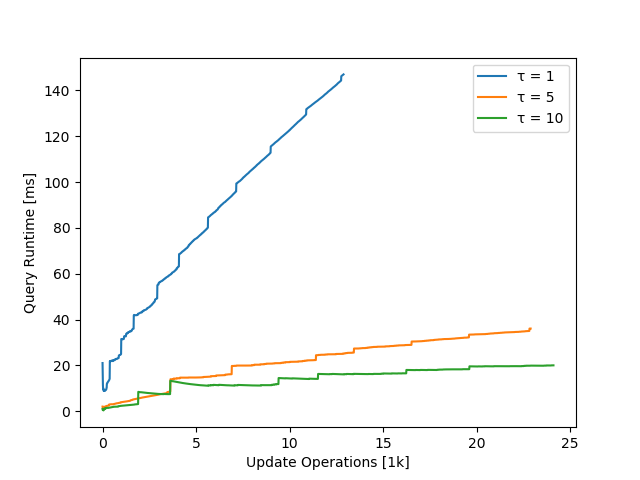
\includegraphics[width=8cm]{query_runtime_taus}
    \caption{}
    \label{fig:query_runtime_taus_synthetic}
  \end{subfigure}
  \begin{subfigure}{0.49\linewidth}
    \centering
    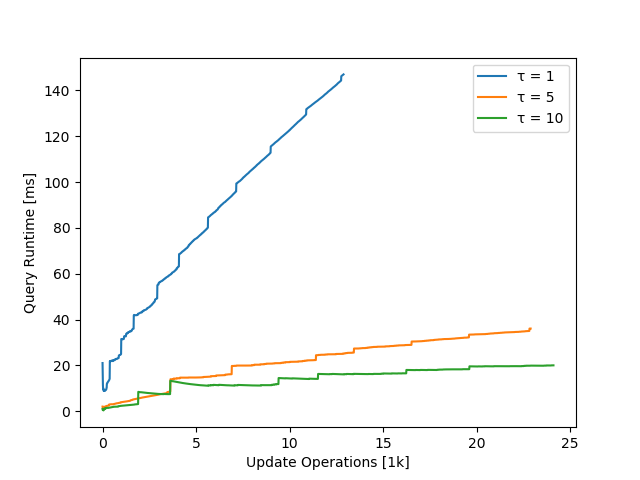
\includegraphics[width=8cm]{query_runtime_taus}
    \caption{}
    \label{fig:query_runtime_taus_aem}
  \end{subfigure}
  \begin{subfigure}{0.49\linewidth}
    \centering
    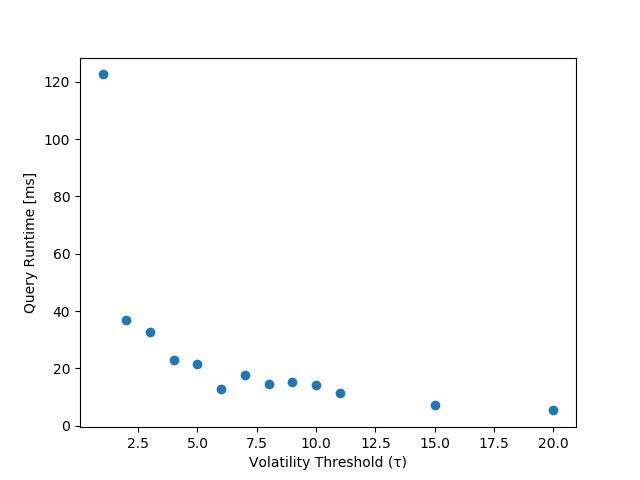
\includegraphics[width=8cm]{tau_query_runtime}
    \caption{}
    \label{fig:tau_query_runtime_synthetic}
  \end{subfigure}
  \begin{subfigure}{0.49\linewidth}
    \centering
    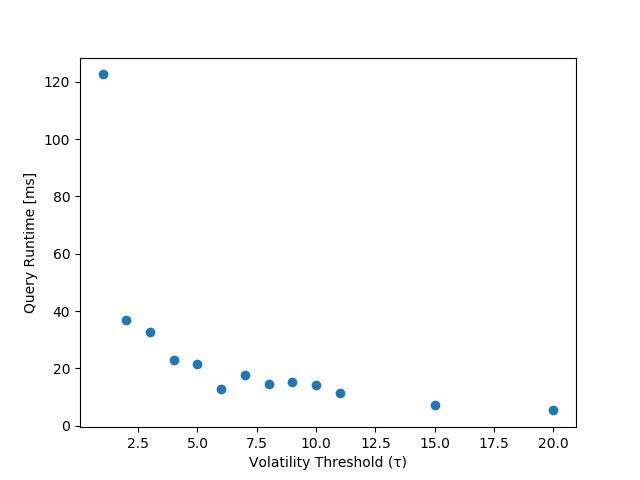
\includegraphics[width=8cm]{tau_query_runtime}
    \caption{}
    \label{fig:tau_query_runtime_aem}
  \end{subfigure}
\caption{Impact of Volatility Threshold $\tau$ on Query Execution Runtime}
\end{figure}

\begin{figure}[h]
  \centering
  \begin{subfigure}{0.49\linewidth}
    \centering
    Synthetic
  \end{subfigure}
  \begin{subfigure}{0.49\linewidth}
    \centering
    AEM
  \end{subfigure}
  \begin{subfigure}{0.49\linewidth}
    \centering
    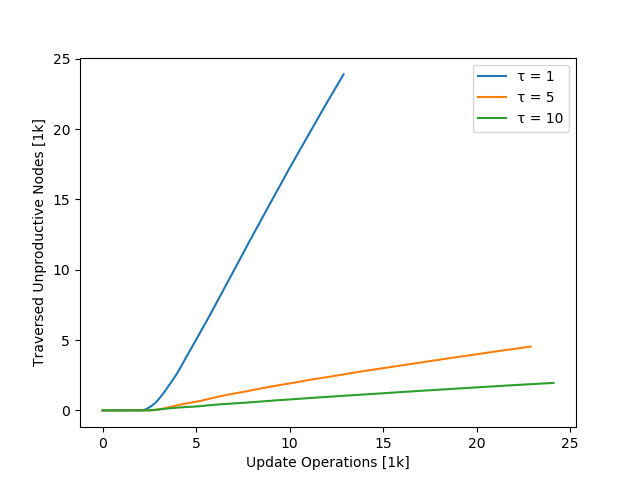
\includegraphics[width=8cm]{traversed_unprod_nodes_taus}
    \caption{}
    \label{fig:trav_unprod_nodes_taus_synthetic}
  \end{subfigure}
  \begin{subfigure}{0.49\linewidth}
    \centering
    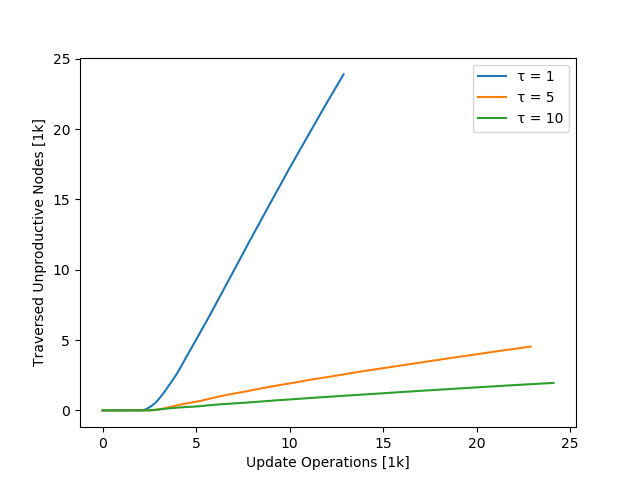
\includegraphics[width=8cm]{traversed_unprod_nodes_taus}
    \caption{}
    \label{fig:trav_unprod_nodes_taus_aem}
  \end{subfigure}
  \begin{subfigure}{0.49\linewidth}
    \centering
    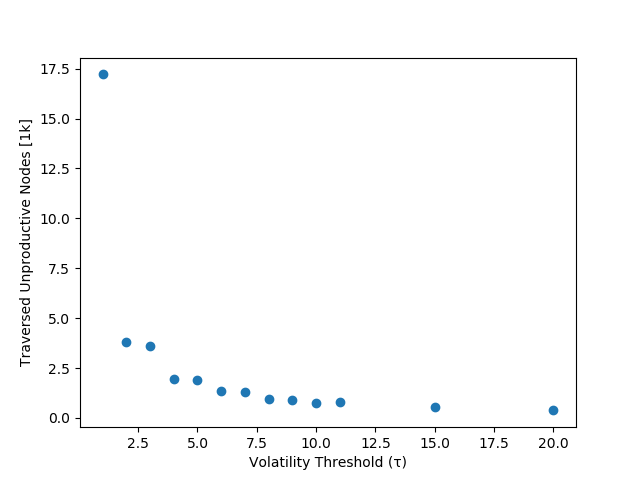
\includegraphics[width=8cm]{tau_unprod_nodes}
    \caption{}
    \label{fig:tau_unprod_nodes_synthetic}
  \end{subfigure}
  \begin{subfigure}{0.49\linewidth}
    \centering
    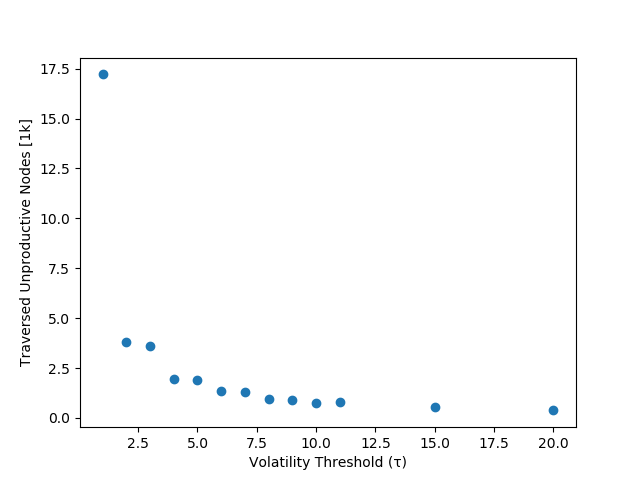
\includegraphics[width=8cm]{tau_unprod_nodes}
    \caption{}
    \label{fig:tau_unprod_nodes_aem}
  \end{subfigure}
  \caption{Impact of Volatility Threshold $\tau$ on Unproductive Nodes}
  \label{fig:volatility_threshold}
\end{figure}

\subsection{Sliding Window Length $L$}

Sliding window length $L$ determines the length of the recent workload that WAPI
considers to compute an index node's volatility count. In this section, we study
the effect of sliding window length $L$ on unproductive nodes and query
execution runtime.

We hyptothesize that an increase in $L$ yields an increase to the number of
traversed unproductive nodes during query execution. If $L$ increases, it is
more likely for a node to become volatile. Having more volatile nodes should
imply an increase in unproductive nodes.

An increase in $L$ yields an increase to the query execution runtime. More
unproductive nodes should increase the number of nodes traversed
during query execution and therefore increase query execution time.

An increase in $L$ yields an increase to the unproductive node density during
query exection. \textbf{Why}

\begin{shaded}
  \begin{itemize}
  \item[$H_6$:] An increase in $L$ yields an inrease to the query execution runtime. 
  \item[$H_7$:] An increase in $L$ yields an increase to the number of
    traversed unproductive nodes during query execution.
  \item[$H_8$:] An increase in $L$ yields an increase to the unproductive node
    density during query execution runtime.
  \end{itemize}
\end{shaded}

\begin{figure}[h]
  \centering
  \begin{subfigure}{0.49\linewidth}
    \centering
    Synthetic
  \end{subfigure}
  \begin{subfigure}{0.49\linewidth}
    \centering
    AEM
  \end{subfigure}
  \begin{subfigure}{0.49\linewidth}
    \centering
    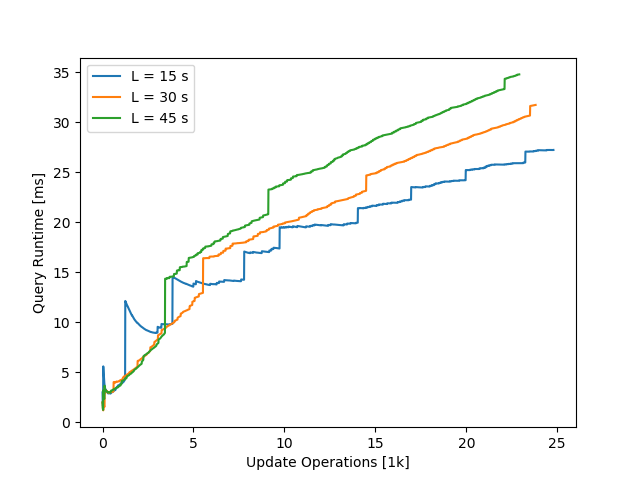
\includegraphics[width=8cm]{query_runtime_Ls}
    \caption{}
    \label{fig:query_runtime_Ls_synthetic}
  \end{subfigure}
  \begin{subfigure}{0.49\linewidth}
    \centering
    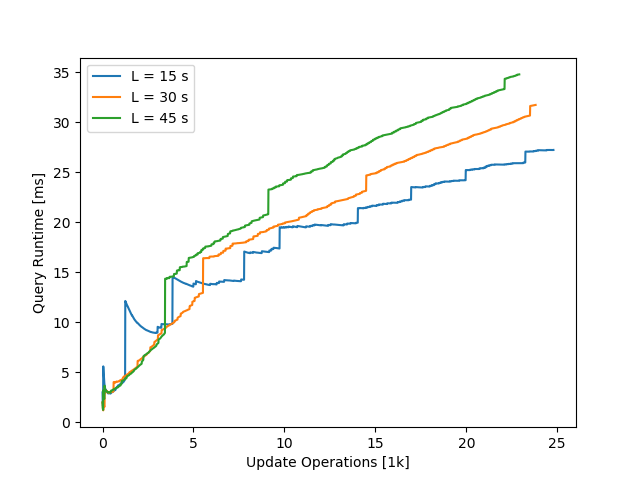
\includegraphics[width=8cm]{query_runtime_Ls}
    \caption{}
    \label{fig:query_runtime_Ls_aem}
  \end{subfigure}
  \begin{subfigure}{0.49\linewidth}
    \centering
    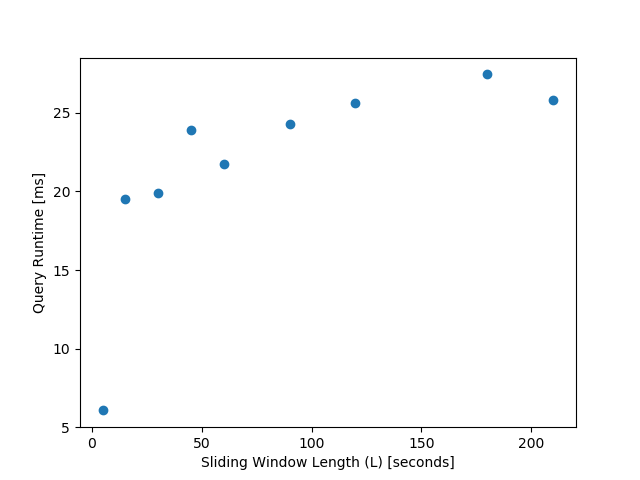
\includegraphics[width=8cm]{L_query_runtime}
    \caption{}
    \label{fig:L_query_runtime_synthetic}
  \end{subfigure}
  \begin{subfigure}{0.49\linewidth}
    \centering
    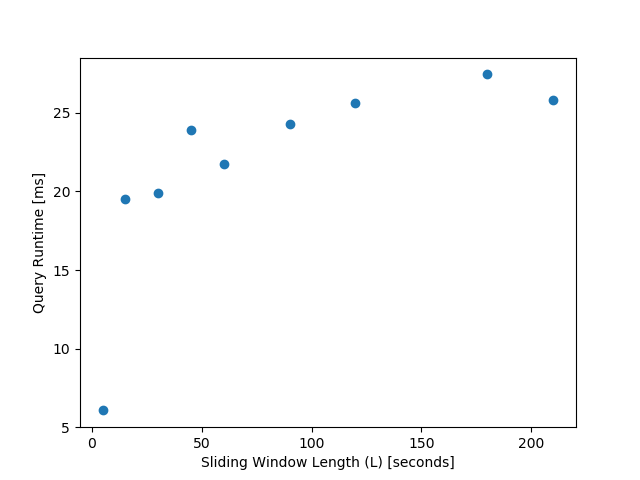
\includegraphics[width=8cm]{L_query_runtime}
    \caption{}
    \label{fig:L_query_runtime_aem}
  \end{subfigure}
  \caption{Impact of Sliding Window Length $L$}
\end{figure}

\begin{figure}[h]\ContinuedFloat
  \centering
  \begin{subfigure}{0.49\linewidth}
    \centering
    Synthetic
  \end{subfigure}
  \begin{subfigure}{0.49\linewidth}
    \centering
    AEM
  \end{subfigure}
  \begin{subfigure}{0.49\linewidth}
    \centering
    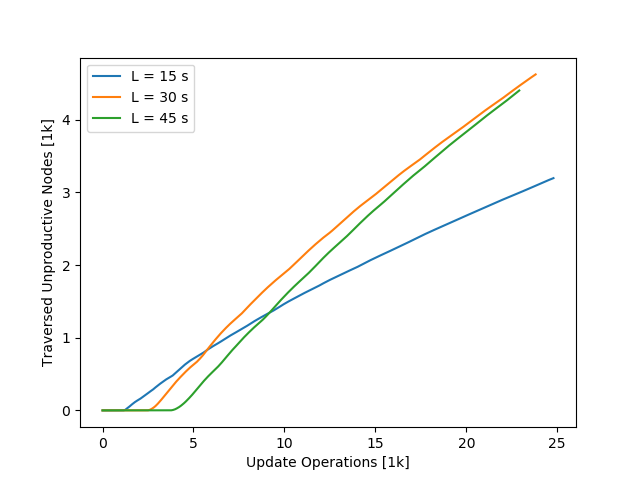
\includegraphics[width=8cm]{traversed_unprod_nodes_Ls}
    \caption{}
    \label{fig:trav_unprod_nodes_Ls_synthetic}
  \end{subfigure}
  \begin{subfigure}{0.49\linewidth}
    \centering
    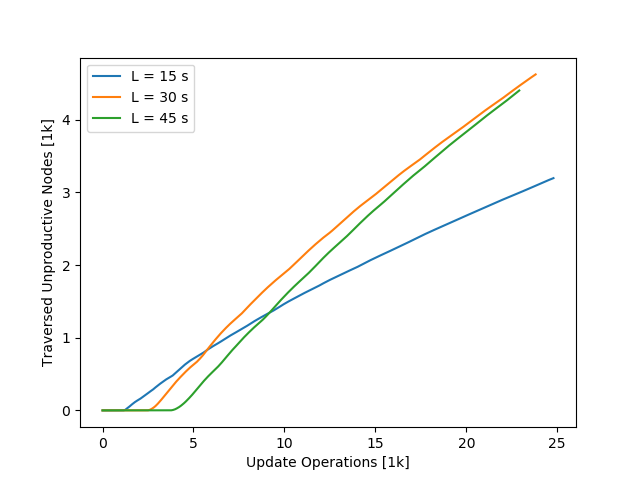
\includegraphics[width=8cm]{traversed_unprod_nodes_Ls}
    \caption{}
    \label{fig:trav_unprod_nodes_Ls_aem}
  \end{subfigure}
  \begin{subfigure}{0.49\linewidth}
    \centering
    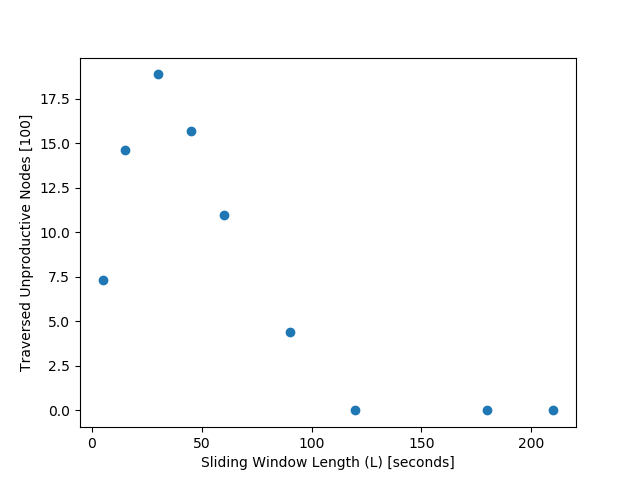
\includegraphics[width=8cm]{L_unprod_nodes}
    \caption{}
    \label{fig:L_unprod_nodes_synthetic}
  \end{subfigure}
  \begin{subfigure}{0.49\linewidth}
    \centering
    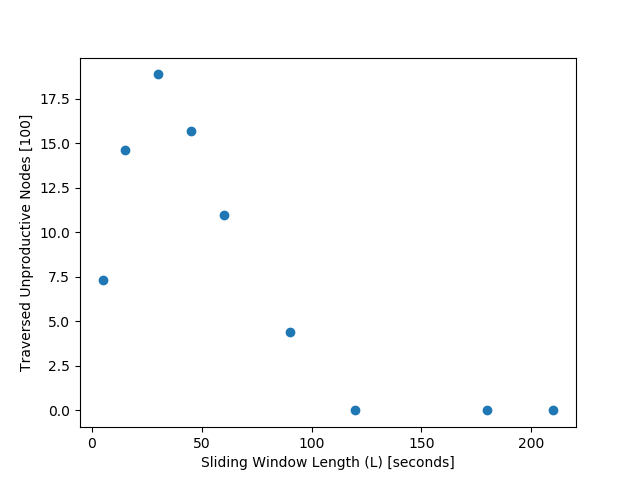
\includegraphics[width=8cm]{L_unprod_nodes}
    \caption{}
    \label{fig:L_unprod_nodes_aem}
  \end{subfigure}
  \caption{Impact of Sliding Window Length $L$ (cont.)}
  \label{fig:sliding_window_length}
\end{figure}

\section{Periodic Garbage Collection (GC)}

\section{Query Time Pruning (QTP)}

\section{Experimental Evaluation}

% In order to empirically evaluate and compare GC and QTP under a changing
% workload, a experiment harness has to be setup.

% datasets

% zipf distribution

% changing Workload

% parameters

\newpage

\bibliographystyle{abbrv}
\bibliography{thesis}

\end{document}
